%\begin{frame}
%\frametitle{Outline}
%    \begin{itemize}
%        \item What Are Generators?
%    \end{itemize}
%\end{frame}

\begin{frame}
    \frametitle{Generators}
    \begin{columns}
    \begin{column}{0.48\paperwidth}
        \begin{itemize}
            \item<1->Suppose that we have some probability space $S$.
            \item<2->$S$ has two variables $X$ (instances) and $Y$ (labels) that
                represent cats and dogs.
            \item<3->Often we want to find a boundary between different types of
                data within a sample space. (Discrimitive Model)
            \item<4->We might instead want to \textit{sample} from this space
                and see what images are here.
            \item<5->Typically we'll only work with a single classification.
        \end{itemize}
    \end{column}
    \begin{column}{0.48\textwidth}
        \includegraphics<1>[width=\textwidth]{SampleSpace_Empty.png}
        \includegraphics<2>[width=\textwidth]{SampleSpace.png}
        \includegraphics<3>[width=\textwidth]{SampleSpace_Classification.png}
        \includegraphics<4>[width=\textwidth]{SampleSpace_Generation.png}
        \includegraphics<5>[width=\textwidth]{SampleSpace_Cats.png}
    \end{column}
    \end{columns}
\end{frame}

\begin{frame}
    \frametitle{Generators}
    \begin{itemize}
        \item In a Discriminitive model we learn a conditional probability
            $P(Y|X)$ (predict the label given an image).
        \item In a Generative model we learn to sample for p(x)
            (produce an image).
        \item<2> In reality we learn $p_\theta(\hat{x})$ from $p_{true}(x)$
    \end{itemize}
\end{frame}

\begin{frame}
    \frametitle{But Why?}
    \includegraphics<1>[width=\textwidth]{ButWhy.jpg}
\end{frame}

\begin{frame}
    \frametitle{But Why?}
    \begin{itemize}
        \item<1-> We can create images that don't exist.
        \item<2-> We can create new datasets.
        \item<3-> We can upscale images/videos.
        \item<4-> We can lean latent variables.
        \item<5-> We can uncover biases.
        \item<6-> And so much more!
    \end{itemize}
\end{frame}

\begin{frame}
    \frametitle{But Why?: Generate Images}
    \begin{columns}
        \begin{column}{0.48\paperwidth}
            \begin{itemize}
                \item We can generate cats that don't exist.
                \item Helps create new data within a dataset.
                \item Can create fake characters/animals/scenes that don't exist
                    in real life but look realistic (art).
            \end{itemize}
        \end{column}
        \begin{column}{0.48\paperwidth}
            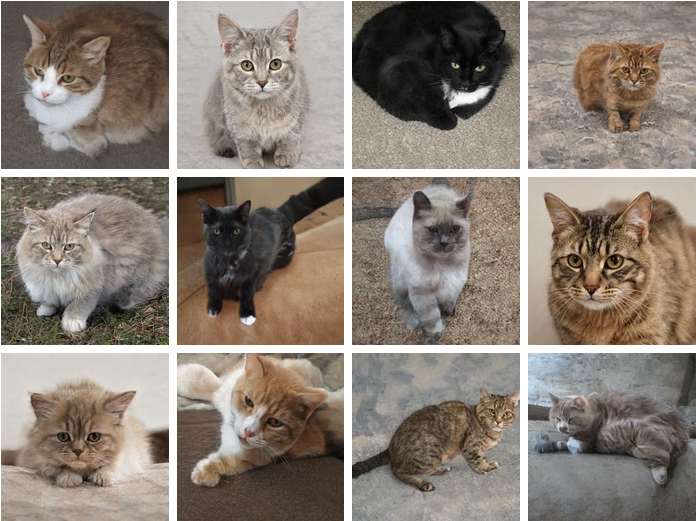
\includegraphics[width=\textwidth]{TCDNE.png}
        \end{column}
    \end{columns}
\end{frame}

\begin{frame}
    \frametitle{But Why?: Upscaling}
    \begin{columns}
        \begin{column}{0.48\paperwidth}
            \begin{itemize}
                \item We can take lossy images and produce higher quality
                    images.
                \item We can also take smaller images and make them larger.
                \item Helpful in compression.
            \end{itemize}
        \end{column}
        \begin{column}{0.48\paperwidth}
            \includegraphics[width=\textwidth]{Upscaling.jpg}
        \end{column}
    \end{columns}
\end{frame}

\begin{frame}
    \frametitle{But Why?: Learn Latent Variables}
    \begin{columns}
        \begin{column}{0.48\paperwidth}
            \begin{itemize}
                \item We can learn the different latent variables in a dataset.
                \item For example we can learn how to make someone old!
                \item We could also use this as a form of compression
                    (autoencoders)
            \end{itemize}
        \end{column}
        \begin{column}{0.48\paperwidth}
            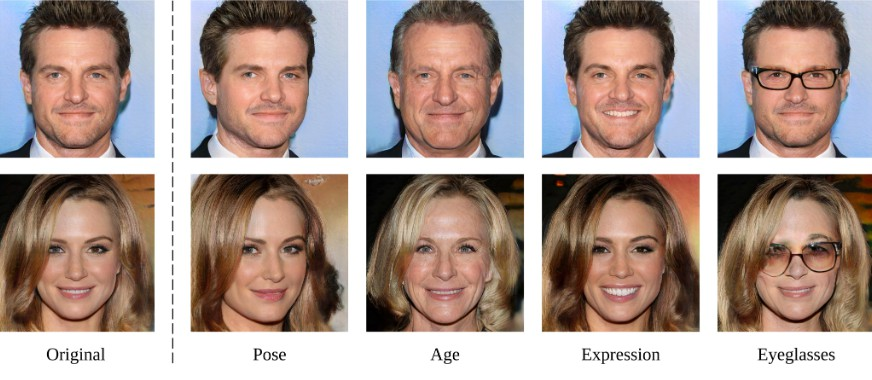
\includegraphics[width=\textwidth]{latent.jpg}
        \end{column}
    \end{columns}
\end{frame}

\begin{frame}
    \frametitle{But Why?: Uncovering Bias}
    \begin{columns}
        \begin{column}{0.48\paperwidth}
            \begin{itemize}
                \item<1-> We have a dataset of faces.
                \item<2-> Might have some distribution, let's say...
                \item<3-> Most of the faces fit in the main part of the
                    distribution.
                \item<4-> We have outliers in the dataset.
                \item<5-> We can now adjust our dataset or potentially generate
                    new images for a classifier if we can't fix the distribution
                    (might not be logistically possible).
            \end{itemize}
        \end{column}
        \begin{column}{0.48\paperwidth}
            \includegraphics<1>[width=\textwidth]{Faces.png}
            \includegraphics<2>[width=\textwidth]{Faces_Distribution.png}
            \includegraphics<3>[width=\textwidth]{Faces_MainDistrib.png}
            \includegraphics<4->[width=\textwidth]{Faces_Tail.png}
        \end{column}
    \end{columns}
\end{frame}


\begin{frame}
    \frametitle{Taxonomy of Generators}
    \includegraphics[width=\textwidth]{taxonomy.png}
    \null\hfill \tiny{source: ian goodfellow}
\end{frame}

\begin{frame}
    \frametitle{Taxonomy of Generators: Implicit Density}
    \begin{columns}
        \begin{column}{0.48\paperwidth}
            \begin{itemize}
                \item We want to learn a stochastic procedure to generate data. 
                \item We learn liklihood-free.
            \end{itemize}
        \end{column}
        \begin{column}{0.48\paperwidth}
            \includegraphics[width=\textwidth]{taxonomy_Implicit.png}
            \null\hfill \tiny{source: ian goodfellow}
        \end{column}
    \end{columns}
\end{frame}

\begin{frame}
    \frametitle{This X Does Not Exist}
    \vspace{-1em}
    \begin{figure}
        \begin{subfigure}{0.25\textwidth}
            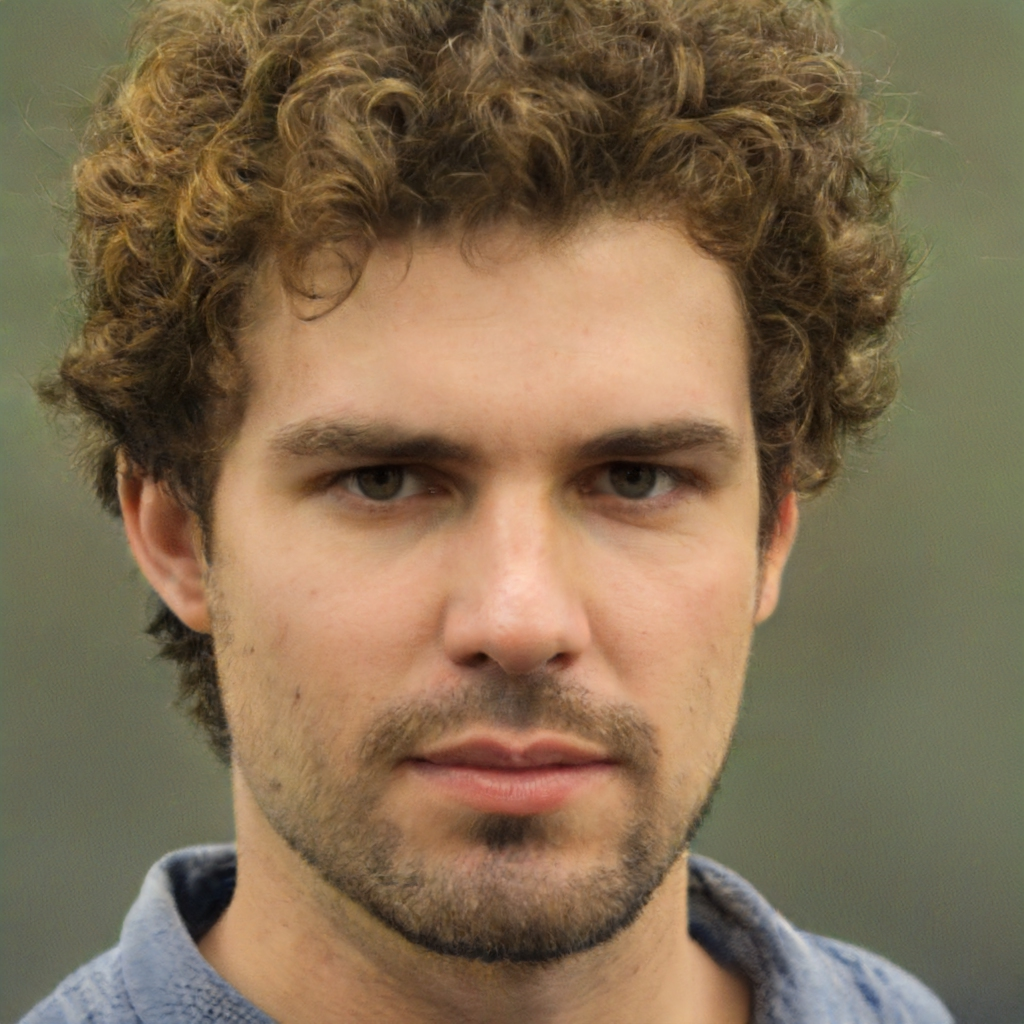
\includegraphics[width=\textwidth]{tpdne.jpg}
            \caption{This Person Does Not Exist (StyleGAN2)}
        \end{subfigure}
        \begin{subfigure}{0.25\textwidth}
            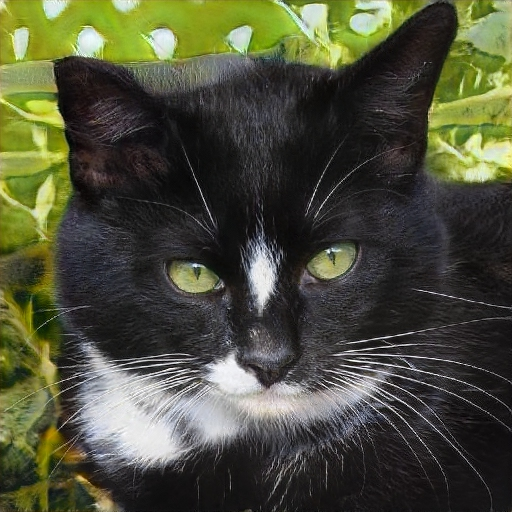
\includegraphics[width=\textwidth]{tcdne.jpg}
            \caption{This Cat Does Not Exist (StyleGAN)}
        \end{subfigure}
        \begin{subfigure}{0.5\textwidth}
            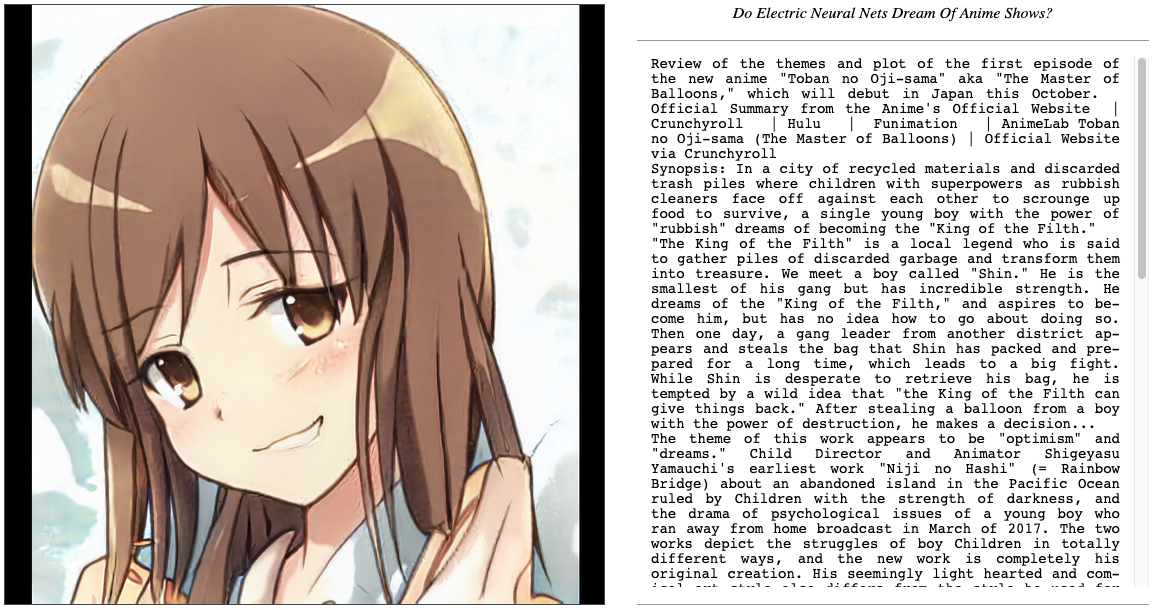
\includegraphics[width=\textwidth]{twdne.png}
            \caption{This Anime Does Not Exist (StyleGAN2 + GPT-3)}
        \end{subfigure}
    \end{figure}
\end{frame}

\begin{frame}
    \frametitle{Generative Adversarial Networks}
    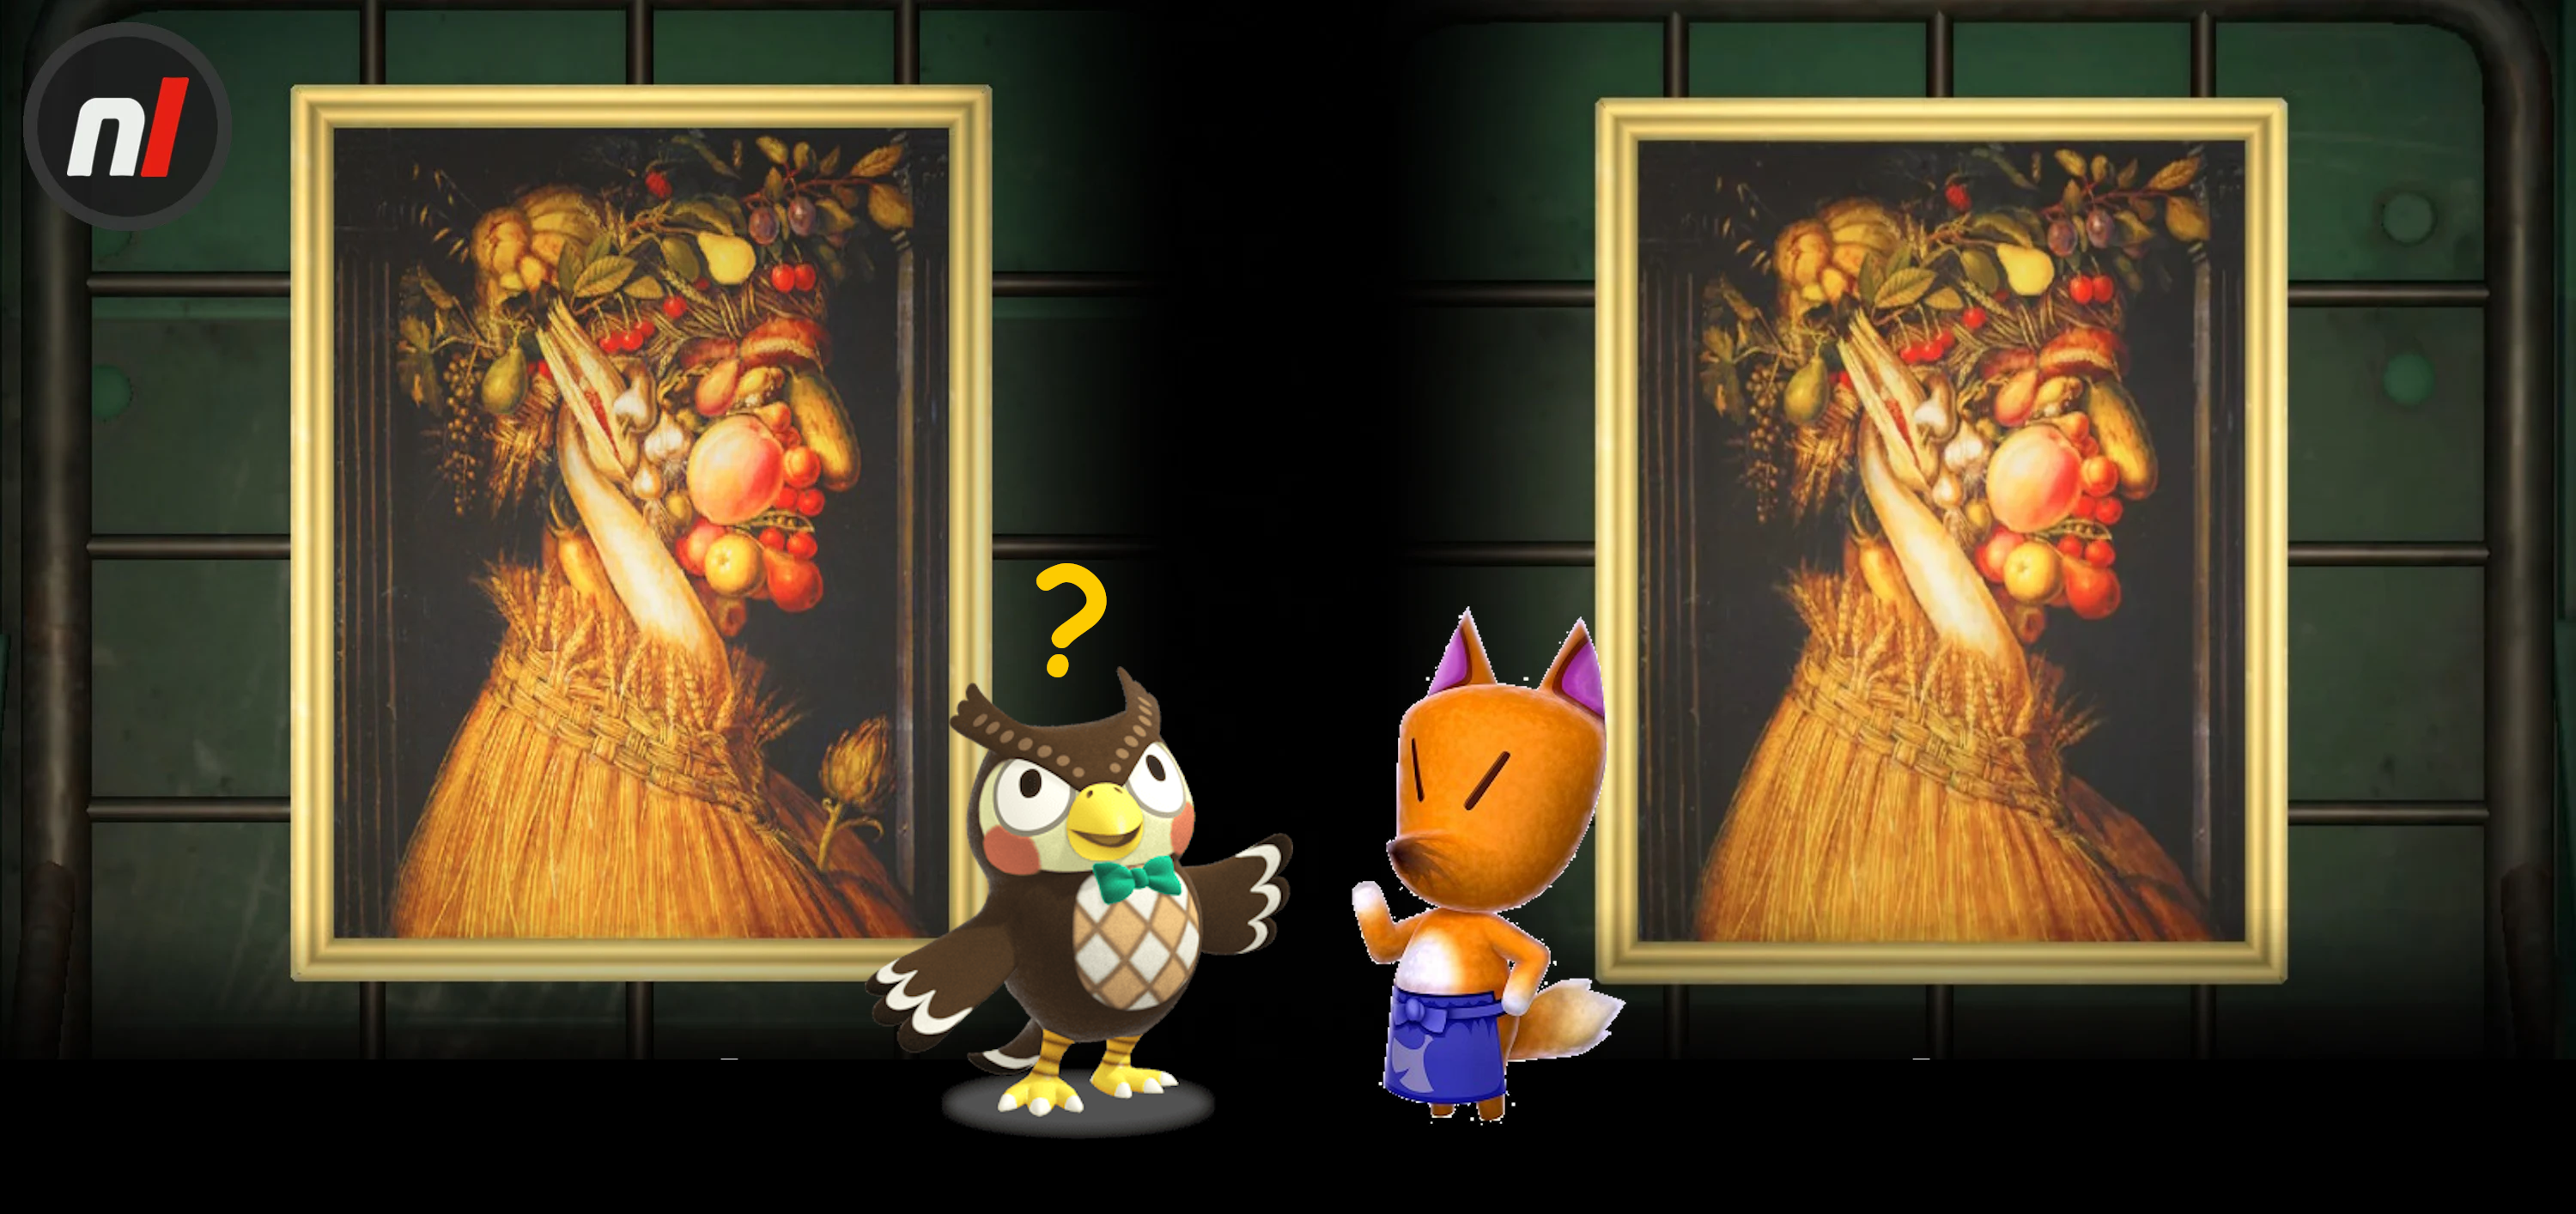
\includegraphics[width=\textwidth]{AC-GAN.png}
\end{frame}

\begin{frame}
    \frametitle{Generative Adversarial Networks}
    \center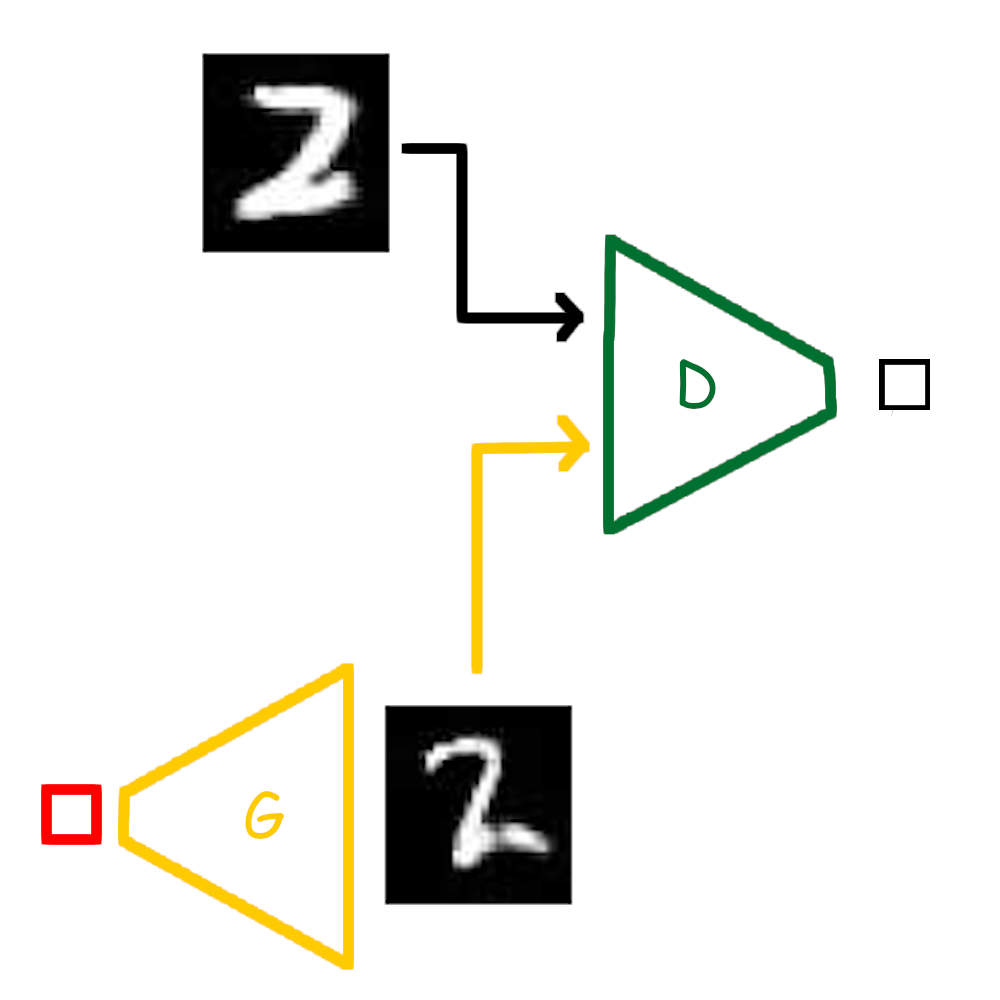
\includegraphics[height=0.75\textheight]{GAN.png}
\end{frame}

\begin{frame}
    \frametitle{Generative Adversarial Networks}
    \center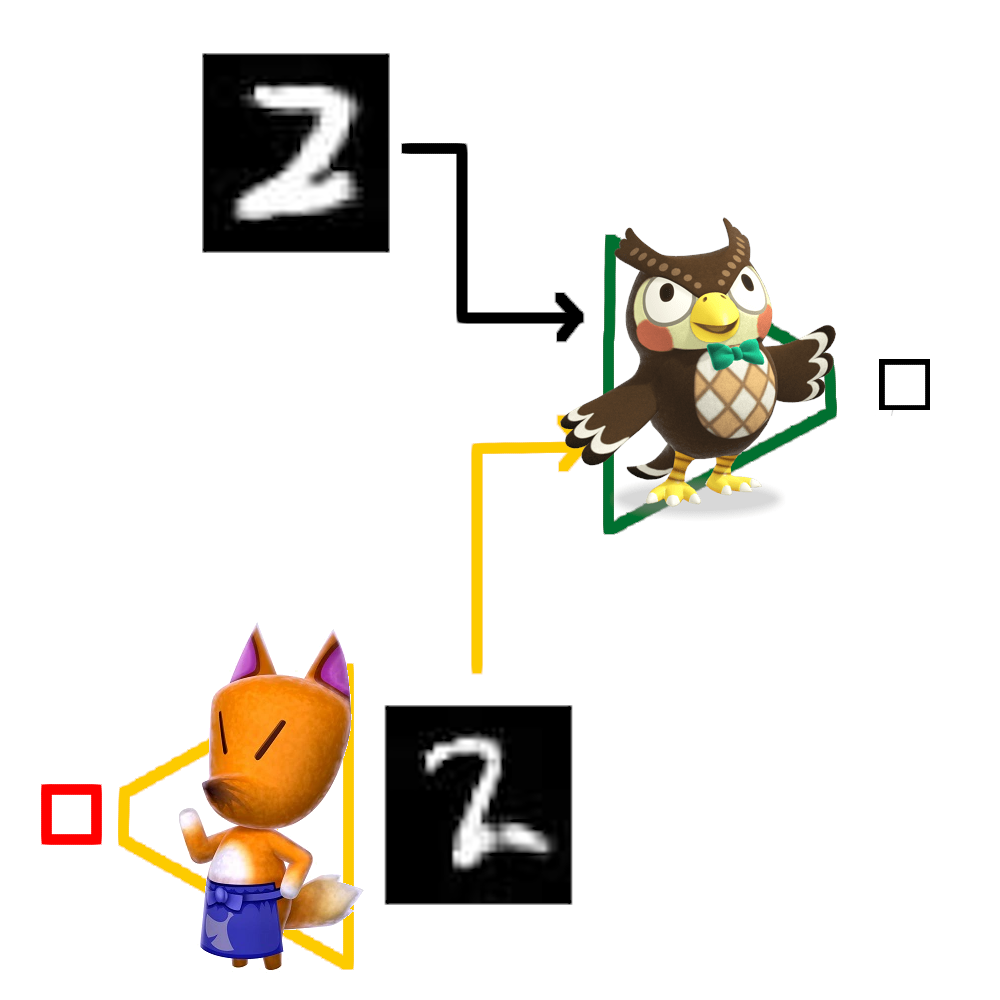
\includegraphics[height=0.75\textheight]{GAN-as-AC.png}
\end{frame}

\begin{frame}
    \frametitle{Generative Adversarial Networks}
    \begin{itemize}
        \item Send noise into Generator.
        \item Send generated image and real images into Discriminator.
        \item Play mini-max game teaching the Generator to fool the
            Discriminator.
        \item When fake image can adaquately fool (a well trained) discriminator
            we produce quality images. 
        \item<2-> In practice we train D, then G then repeat. 
    \end{itemize}
\end{frame}

\begin{frame}
    \frametitle{But Why Is This Implicit?}
    \begin{itemize}
        \item We didn't learn a density function.
        \item We just focus on generating samples.
        \item Don't have an (easy) smooth transition between latent variables.
        \item "We're training them to memorize, not generalize" - Ian Goodfellow
    \end{itemize}
\end{frame}

\begin{frame}
    \frametitle{Taxonomy of Generators: Explicit Density}
    \begin{columns}
        \begin{column}{0.48\paperwidth}
            \begin{itemize}
                \item We want to learn a distribution of
                    data. 
                \item We assume some prior about the distribution of the data. 
                \item We learn the log-liklihood of the function $\log
                    p_\theta(x)$
            \end{itemize}
        \end{column}
        \begin{column}{0.48\paperwidth}
            \includegraphics[width=\textwidth]{taxonomy_Explicit.png}
            \null\hfill \tiny{source: ian goodfellow}
        \end{column}
    \end{columns}
\end{frame}

\begin{frame}
    \frametitle{AutoEncoders}
    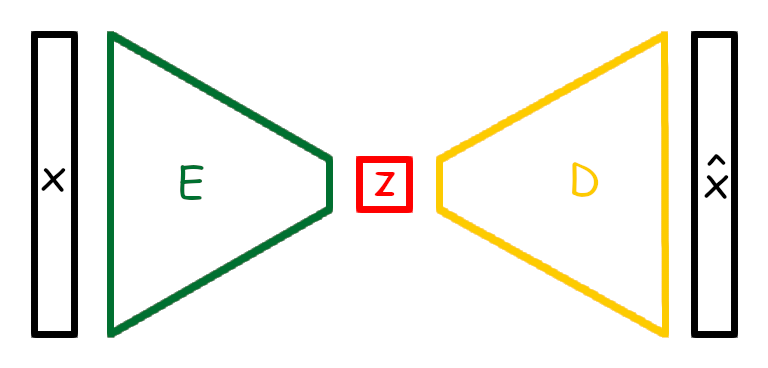
\includegraphics[width=\textwidth]{AutoEncoder.png}
\end{frame}


\begin{frame}
    \frametitle{AutoEncoders}
    \begin{columns}
        \begin{column}{0.48\paperwidth}
            \begin{itemize}
                \item Want to learn latent variable $z$ from $x$. $\mathbb{R}^n
                    \mapsto \mathbb{R}^m$ where $m<n$
                \item Compressed representation of the data.
                \item Since we don't have training data for z, we construct a
                    decoder to do unsupervised learning.
            \end{itemize}
        \end{column}
        \begin{column}{0.48\paperwidth}
            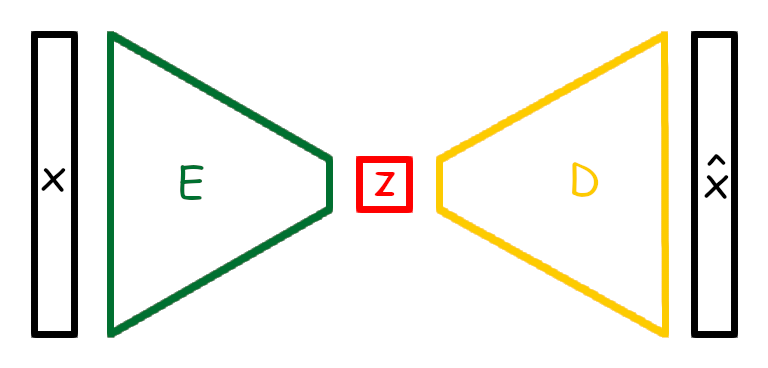
\includegraphics[width=\textwidth]{AutoEncoder.png}
        \end{column}
    \end{columns}
\end{frame}

\begin{frame}
    \frametitle{AutoEncoders}
    \begin{columns}
        \begin{column}{0.48\paperwidth}
            \begin{itemize}
                \item<1-> Want to take $x$ and produce $\hat{x}$
                \item<2-> Sample $x$ from dataset and encode to latent space
                    $z$.
                \item<3-> Decode to sample from $z$ and generate $\hat{x}$
                \item<4-> Regularize $||x-\hat{x}||^2$
                \item<5-> Gives us a unsupervised training.
            \end{itemize}
        \end{column}
        \begin{column}{0.48\paperwidth}
            \includegraphics<1>[width=\textwidth]{AutoEncoder_blank.png}
            \includegraphics<2>[width=\textwidth]{AutoEncoder_In.png}
            \includegraphics<3>[width=\textwidth]{AutoEncoder_Out.png}
            \includegraphics<4->[width=\textwidth]{AutoEncoder_Reg.png}
        \end{column}
    \end{columns}
\end{frame}

\begin{frame}
    \frametitle{Pick Our Latent Space Size Carefully}
    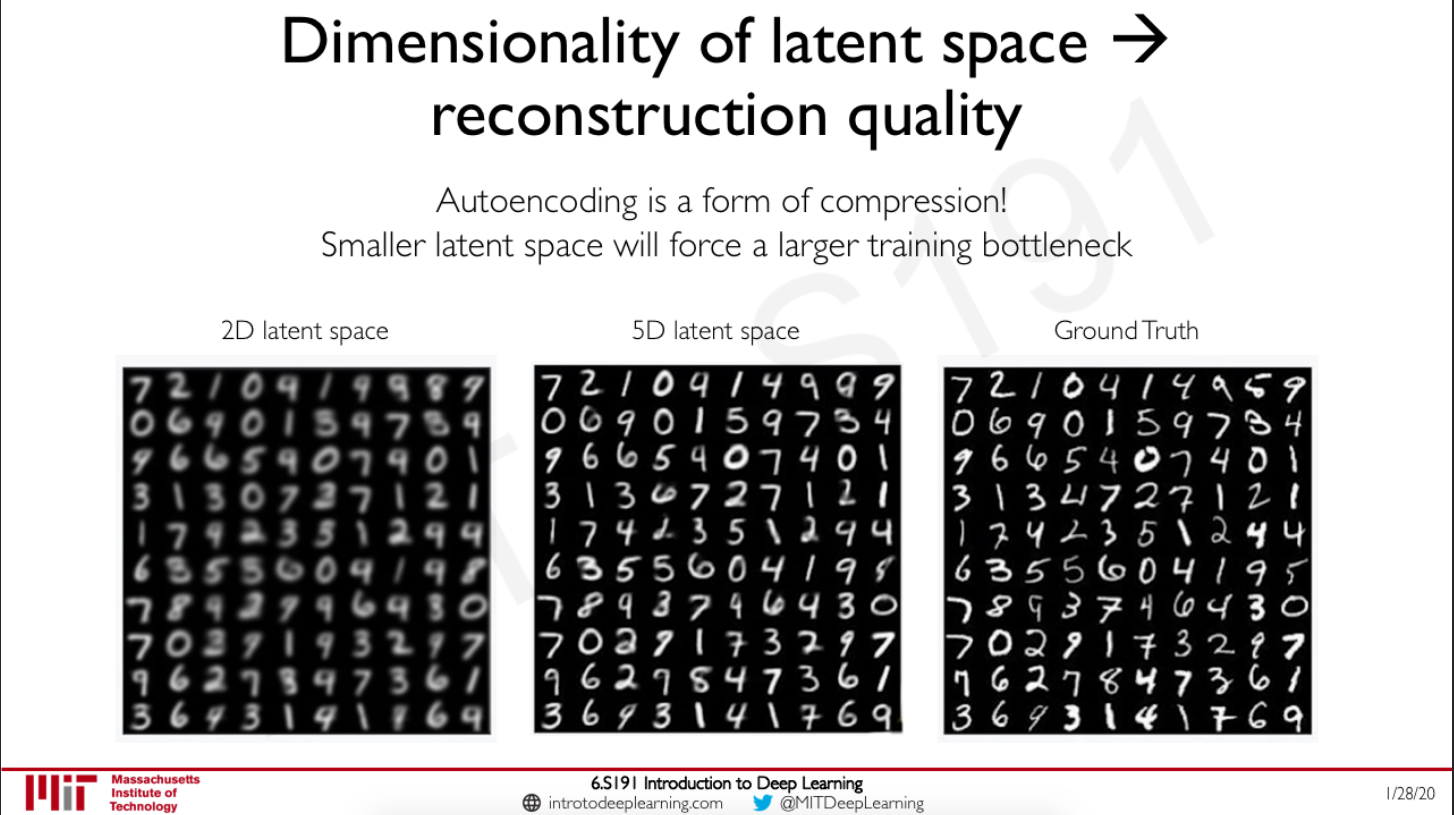
\includegraphics[width=\textwidth]{AE-MNIST.png}
\end{frame}
